\chapter{Uczenie motywowane}
\label{cha:rozdzial2}

Człowiek od momentu, kiedy jest wstanie poznawać swoje środowisko, w którym się 
znajduje ma ochotę eksplorować na swoje możliwości. Małe dzieci, które nie 
umieją jeszcze chodzić albo raczkować, mogą tworzyć skojarzenia pomiędzy 
różnymi czynnikami. Jednym z przykładów może być nawet karmienie takiego 
dziecka małą butelką i poprzez umożliwianie mu trzymanie tej butelki 
samodzielnie, małe dziecko będzie w stanie po pewnym czasie utworzyć 
skojarzenie, że jeżeli będzie trzymało mocno butelkę i w odpowiedniej pozycji, 
to będzie mogło zjeść w razie głodu.

Eksploracja środowiska i swobodne poznawanie go, umożliwia tworzenie połączeń 
asocjacji pomiędzy pewnymi obserwacjami, akcjami jakie wykonaliśmy na nich oraz 
rezultatów jakie zostały otrzymanie w wyniku takich a nie innych akcji. Innym 
przykładem u małego człowieka jest to, że niepilnowane młode dziecko może 
dotknąć czegoś gorącego i się oparzyć, mimo, że rodzice zabronili tego. Dopiero 
poczucie fizycznego bólu sprawi, że dziecko będzie dobrze pamiętało, żeby 
więcej tego nie robić. Dlatego też człowiek często uczy się na własnych błędach 
najlepiej, kiedy sam czegoś doświadczy.

Kluczowe dla uczenia motywowanego (ang. \textit{motivated learning}) jest 
pojęcie motywacji w ucieleśnionej inteligencji (ang. \textit{motivation in 
embodied intelligence}). Inteligencja ucieleśniona jest obliczeniowym 
podejściem do projektowania i rozumienia inteligentnego zachowania u 
ucieleśnionych agentów poprzez wzięcie pod uwagę ścisłego powiązania między 
agentem, a jego otoczeniem. Należy brać pod uwagę jego ograniczenia tj. 
ograniczenia własnego ciała (ograniczenia mechaniczne i/lub elektryczne 
robota), systemu percepcyjnego (systemy wizyjne i ich sprzętowe ograniczenia) 
oraz motoryczne. Jedną z najbardziej wpływowych postaci w procesie 
projektowania ucieleśnionej inteligencji jako metodologii był Rodney Brooks. 
Zasugerował on tworzenie inteligentnych maszyn poprzez interakcję ze 
środowiskiem napędzane przez percepcję i akcję niż przez konkretne 
wyspecjalizowany algorytm.

W dzisiejszy czasach badania w zakresie sztucznej inteligencji są kojarzone z 
wyspecjalizowanym rozwiązywaniem problemów tj. reprezentacja wiedzy, 
zrozumienie języka naturalnego czy oglądanej sceny czy odpowiadanie na pytania. 
Wszystkie te zagadnienia są bardzo ciekawe i sprawiają, że wiele problemów 
zostaje rozwiązywane przez komputery. Jednak nie ma w nich systemu, który spaja 
wszystkie te zagadnienia w jeden system, który mógłby być określaną "silną 
inteligencją".

\section{Definicje związane z projektowaniem ucieleśnionej inteligencji}

W celu projektowania maszyn ucieleśnionej inteligencji zostały zdefiniowane 
pewne zasady i założenia. Pierwszym z nich było to, że agent rozwija się w 
zmieniającym środowisku, które może manipulować i postrzegać korzystając z 
dostępnych sensorów. Nie istnieje potrzeba tworzenia modelu środowiska, 
ponieważ ono się może zmieniać. 

Dodatkowe reguły projektowania zostały zawarte w \cite{pfeifer_ei}:
\begin{enumerate}
	\item Reguła taniego projektu i nadmiarowości -- projekt maszyny powinien 
	być prosty i jego projekt sprawiał, że funkcjonalności podzespołów nachodzą 
	na siebie pozwalając na działanie maszyny w razie awarii jakiegoś 
	podzespołu.
	\item Reguła równoległych, luźno związanych procesów -- ta reguła wymusza 
	na maszynie to, że inteligencja pojawia się przez interakcję 
	niskopoziomowych procesów np. sterowania ramionami ze środowiskiem.
	\item Reguła wartości -- reguła ta może wymuszać, aby maszyna robiła, to co 
	jest dobre dla niej. Umożliwia ona sugerowanie maszynie, co powinna zrobić 
	w danej sytuacji (agenty uczenia ze wzmocnieniem uczą się korzystając m.in. 
	z tej reguły)
\end{enumerate}
		
\section{Inteligencja}
Do dzisiaj nie ma dokładnej definicji inteligencji. Jest wiele interpretacji, a 
jednocześnie należy mieć na uwadze, aby nie mylić inteligencji ze złożonym 
zachowaniem. To bardzo ważne, ponieważ możemy wziąć pewien algorytm, np. 
szukania najkrótszej ścieżki w grafie, która ogółem jest złożonym problemem, 
który składa się ze skończonej liczby kroków. Zdecydowanie nie można 
stwierdzić, że ten algorytm jest inteligenty. To tylko pewien zbiór prostych 
czynności, które rozwiązują konkretny problem i użyte do czegoś innego (można 
tak nazwać zmieniające się środowisko), na pewno nie da dobrych rezultatów.

Opisy inteligencji skupiają się na opisie właściwości umysły, niż samym umyśle. 
W swojej pracy \cite{stewart_93} John Stewart zdefiniował systemy kognitywne 
jako:

\textbf{Definicja:} System jest kognitywny wtedy i tylko wtedy, gdy wejścia z 
sensorów powodują akcje w konkretny sposób, tak aby spełnić wymagania do 
przeżycia w środowisku. 


\textbf{Definicja:} Uczeleśniona inteligencja (ang. \textit{embodied 
intelligence} EI) jest zdefiniowana jako mechanizm, który uczy się jak 
przetrwać we wrogim środowisku (wrogie można także określić jako zmieniające 
się).

Ta druga definicja odnosi się do wszystkich form ucieleśnionej inteligencji: 
biologicznej, mechanicznej czy wirtualnych agentów. Wynika z tego, że agent EI 
wchodzi w interakcje ze środowiskiem i postrzega wprowadzone zmiany poprzez 
sensory. Agent musi się nauczyć jak przetrwać w środowisku. Natomiast wrogość 
środowiska może być określana na różne sposoby. Może to być jego ciągła 
zmienność, czy mała dostępność surowców potrzebnych agentowi przetrwania. Ważne 
jest to, że ta wrogość jest stała. Przykładowo, poziom naładowania baterii jest 
stałych zagrożeniem dla agenta. Jeżeli poziom naładowania będzie się 
zmniejszał, to dyskomfort wywoływany przez sensor odpowiedzialny za pomiar 
baterii będzie rósł.

Kolejnym ważnym elementem definicji ucieleśnionej inteligencji jest aspekt 
uczenia. Jeżeli agent wie jak przetrwać we wrogim środowisku, ale nie wie jak 
się nauczyć nowych umiejętności, nie jest inteligentny. Przykładowo, algorytm, 
która zajmuje się sterowaniem jakiegoś procesu technologicznego nie jest 
inteligentny, ponieważ nie będzie w stanie nauczyć się sterować samochodem. W 
zamierzeniu jego zadaniem było regulowanie wartości zadanej konkretnego procesu 
technologicznego.

Należy zwrócić uwagę, że EI odróżnia wiedzę od inteligencji. Wiedza może być w 
pewien sposób zintegrowana z agentem w trakcie jego projektowania, np. jako 
zbiór pewnych reguł zachowania. Natomiast inteligencja sprawia, że ta wiedza 
może być użyta do tworzenia nowych umiejętności i zarządzania nimi w sposób 
zorganizowany i koherentny.

\section{Projektowanie ucieleśnionej inteligencji}

Uczenie jest aktywnym procesem. Informacje o otoczeniu EI zdobywa poprzez 
koordynację pary sensor -- motor. Uczenie się, które akcje są pożądane, a które 
nie, sprawiają, że agent uczący jest lepiej przystosowany do wrogiego 
środowiska. Można odróżnić co najmniej dwa sposoby na adaptowanie do zmiennego 
środowiska \cite{motivation_in_ei}:

\begin{enumerate}
	\item ewolucyjne -- naturalna selekcja agentów (gatunków zwierząt), które 
	są najlepiej przystosowane lub rozwój nowych umiejętności np. pocenie się, 
	aby utrzymać odpowiednią temperaturę,
	
	\item kognitywne -- poprzez uczenie, używając pamięci i asocjacji, stosując 
	rozpoznawanie schematów, budowanie reprezentacji i implementowanie celów.
\end{enumerate}

Schematy na wielu poziomach abstrakcji są uczone i zapamiętywane przez agenta. 
Pewne abstrakcyjne reprezentacje są budowane aby reprezentować akcje i 
umiejętności. Cała struktura wzorów i relacji pomiędzy nimi jest reprezentowana 
w pewnej postaci w pamięci, która jest asocjacyjna i epizodyczna. Ten system 
jest rozproszony, nadmiarowy i równoległy a dodatkowo krótko i długoterminowy. 
Cały ten system łączy się ze sobą i wchodzi w interakcję w czasie rzeczywistym.

Krytycznym aspektem rozwoju umysłu człowieka jest samoorganizacja. Dzięki niej 
neurony mogą szybko tworzyć nowe reprezentacje zapamiętanych schematów, uczyć 
się jak wchodzić w interakcję z otoczeniem oraz budować oczekiwania związane z 
przyszłymi wydarzeniami, czyli umiejętność prognozowania przyszłych wydarzeń na 
podstawie aktualnego stanu oraz tego, co stało się w przeszłości.

Agent uczenia motywowanego dzieli wspólne właściwości ze specjalnym typem 
agenta racjonalnego (ang. \textit{rational software agent}) znanego jako agenta 
przekonań -- pragnień -- intecji (ang. \textit{belief -- desire -- intention}). 
To pewien z modeli tworzenia oprogramowania, który umożliwia rozdzielenie 
funkcjonalności od siebie. Ten model skupia się na planowaniu i sposobie 
wykonania pewnych zadań. Cechy wspólne z agentem uczenia motywowanego to 
tworzenie reprezentacji poznanego środowiska, pragnienia to motywacje dla 
agenta motywowanego. Różnicą jest sposób implementacji reprezentacji wiedzy. 
Dla agenta uczenia motywowanego nie ma konkretnego sposobu implementacji, 
ponieważ widza ta jest reprezentowana przez struktury sieci neuronowych a tym 
samym wszelkie plany, co do wykonywanych akcji muszą być pochodzą z aktywacji 
neuronów w sieci neuronowej.


\section{Ból jako motywacja}

Zadaniem każdej maszyny jest wykonywanie pewnych z góry określonych zadań. 
Pytaniem jest, co może być motywujące, aby dana maszyna/program wykonywały go w 
sposób perfekcyjny. Dla pewnych grup algorytmów można zdefiniować z góry 
określoną funkcję kosztu, którą w sposób iteracyjny usprawnia działanie danego 
algorytmu. Jednakże takie podejście daje bardzo mało możliwości do 
generalizowania zdobytych umiejętności na nowe potrzeby, np. zmiennego 
środowiska.

Aby odpowiedzieć na pytanie, co może motywować maszyny do ulepszania swoich 
możliwości w sposób bardziej zgeneralizowany, można zastanowić się, co motywuje 
ludzi do rozwijania swoich umiejętności. Próbą odpowiedzi na to pytanie podjął 
się psycholog Csíkszentmihályi w książce opisującej teorię przepływu 
\cite{csikszentmihalyi1996creativity}. W tej teorii opisano, że ludzie 
otrzymują wewnętrzne nagrody za wszelkie aktywności, które są trochę ponad ich 
aktualny poziom rozwoju. 

Starzyk w pracy \cite{motivation_in_ei} sugeruje, że to wrogość środowiska, 
które jest ujęte w definicji agenta ucieleśnionej inteligencji (EI) jest 
najbardziej efektywnym czynnikiem motywującym do uczenia. Ma to odniesienie do 
ludzkiego sposobu uczenia. Podstawowym bólem może być ciekawość. To ona 
sprawia, że chcemy poznawać nowe rzeczy. Dla małego dziecka taka ciekawość może 
wywołać ból fizyczny, kiedy z ciekawości oparzy się dotykając czegoś gorącego. 
Ale ten ból sprawi, że w przyszłości będzie wiedziało jak postępować, aby nie 
zwiększać tego bólu.

Według Starzyka bóle prymitywne są bezpośrednio związane z bodźcami odbieranymi 
przez sensory maszyny. Natomiast definiuje on bóle abstrakcyjne (ang. 
\textit{abstract pains}). Pojawiają się one, kiedy agent nie jest w stanie 
wykonać akcji, która zmniejszy wartość bólu prymitywnego. W ten sposób mogą się 
tworzyć struktury grafowe opisujące relacje pomiędzy różnymi bólami. Co ważne, 
bóle abstrakcyjne nie są stymulowane przez sensor wartości fizycznej, np. niski 
poziom naładowania baterii dla robota.  
\ref{fig:abstractpainscreation}.

\begin{figure}[H]
	\centering
	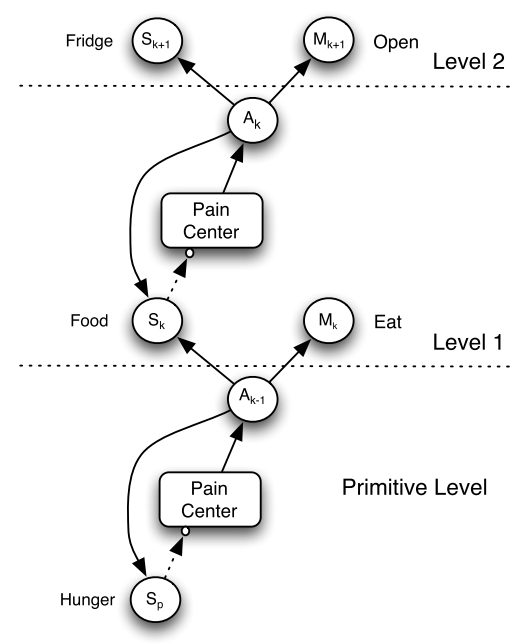
\includegraphics[width=0.5\linewidth]{rozdzial2/images/abstract_pains_creation}
	\caption{Tworzenie sygnałów abstrakcyjnych bóli. Źródło: 
	\cite{ml_dev_auto_systems}}
	\label{fig:abstractpainscreation}
\end{figure}

Bóle tworzą hierarchię wszerz i wgłąb, tworząc struktury grafowe. 
W takich strukturach teoretycznie mogą pojawiać się zamknięte ścieżki, np. brak
jedzenia może sprawić, żeby kupić więcej jedzenia, a do tego potrzebne są 
pieniądze, które można zdobyć sprzedając jedzenie. Należy wziąć pod uwagę takie 
sytuacje w procesie tworzenia całej architektury i sposobu uczenia maszyny.

\section{Tworzenie celów w uczeniu motywowanym}

Jednym z podstawowych źródeł tworzenia nowych celów jest wcześniej wspomniany 
ból. Najbardziej prymitywnym bólem u ludzi jest uczucie dyskomfortu, gdy czują 
głów. W maszynach można to odnieść do poziomu naładowania baterii w robocie i 
coraz niższy poziom sprawia, że ból związany z brakiem energii zwiększa się. 
Agent uczenia motywowanego musi się nauczyć jak ten ból zmniejszać, tak jak 
człowiek uczy się zdobywać jedzenie oraz jeść. Mimo, że wszelkie abstrakcyjne 
bóle, które wykształcają się w dalszym rozwoju, to te prymitywne umożliwiają 
realizację kolejnych zadań czy celów.

Dokładny opis algorytmu tworzenia celów został opisany w 
\cite{ml_comp_int}

\textbf{Algorytm tworzenia celów (ang. \textit{goal creation system})}
\begin{enumerate}
    \item Wybierz dominujący ból stosując regułę zwycięzca bierze wszystko 
        (ang. \textit{winner takes all}) spomiędzy konkurujących ośrodków bólu.
        \begin{itemize}
            \item Jeżeli żaden z bóli nie przekracza wcześniej zdefiniowanego 
                progu, czekaj aż któryś z nich przekroczy ten próg.
        \end{itemize}
    \item Jako aktualny cel wybierz zmniejszenie dominującego bólu.
        \begin{itemize}
            \item aktualny cel motywuje agenta do działania.
        \end{itemize}
    \item Wybierz wcześniej nauczoną akcje, która z najwyższym 
          prawdopodobieństwem spełni aktualny cel.
        \begin{itemize}
            \item Jeżeli nie ma żadnego, idź do punktu 6.
        \end{itemize}
    \item Sprawdź czy wybrana czynność może być wykonana w aktualnym środowisku. 
        Jeśli nie, idź do punktu 3.
    \item Wykonaj akcję.
        \begin{itemize}
            \item Jeśli ta akcja \textit{obniżyła} wartość dominującego bólu:
                \begin{enumerate}
                    \item Zwiększ wartości wag zależności pomiędzy aktualnym 
                        bólem a~akcją jaka została wykonana i~zwiększ wartość 
                        wag odpowiadających abstrakcyjnemu bólowi powiązanego 
                        z~tą akcją.
                    \item Idź do punktu 1.
                \end{enumerate}
            \item Jeśli ta akcja \textit{nie obniżyła} wartości dominującego bólu.
                \begin{enumerate}
                    \item Zmniejsz wartości wag zależności pomiędzy aktualnym 
                        bólem a~akcją jaka została wykonana i~zmniejsz wartość 
                        wag odpowiadających abstrakcyjnemu bólowi powiązanego 
                        z~tą akcją.
                    \item Idź do punktu 3.
                \end{enumerate}
        \end{itemize}
    \item Wykonaj eksplorację przestrzeni akcji mającą na celu spełnienie celu.
        \begin{itemize}
            \item Jeśli nowa akcja \textit{zmniejszyła} wartość dominującego bólu.
                \begin{enumerate}
                    \item Zwiększ wartości wag zależności pomiędzy aktualnym 
                        bólem a~akcją jaka została wykonana i~stwórz nowy 
                        abstrakcyjny ból związany z~niemożliwością wykonania 
                        tej akcji.
                    \item Idź do punktu 1.
                \end{enumerate}
            \item Jeśli nowa akcja \textit{nie zmniejszyła} wartości 
                dominującego bólu, idź do punktu 6.
        \end{itemize}
\end{enumerate}

Uczenie motywowane może być zastosowane wspólnie z~uczeniem opartym na 
ciekawości (ang. \textit{curiosity based learning}) -- ciekawość poinformuje 
agenta o~nowych odkryciach, podczas gdy uczenie motywowane skupi się na 
poszukiwaniu konkretnych celów, które nie są podane przez twórcę (tak jak 
w~uczeniu ze wzmocnieniem).

\section{Podstawowy element systemy tworzenia celów}

Tekst

\begin{figure}[H]
	\centering
	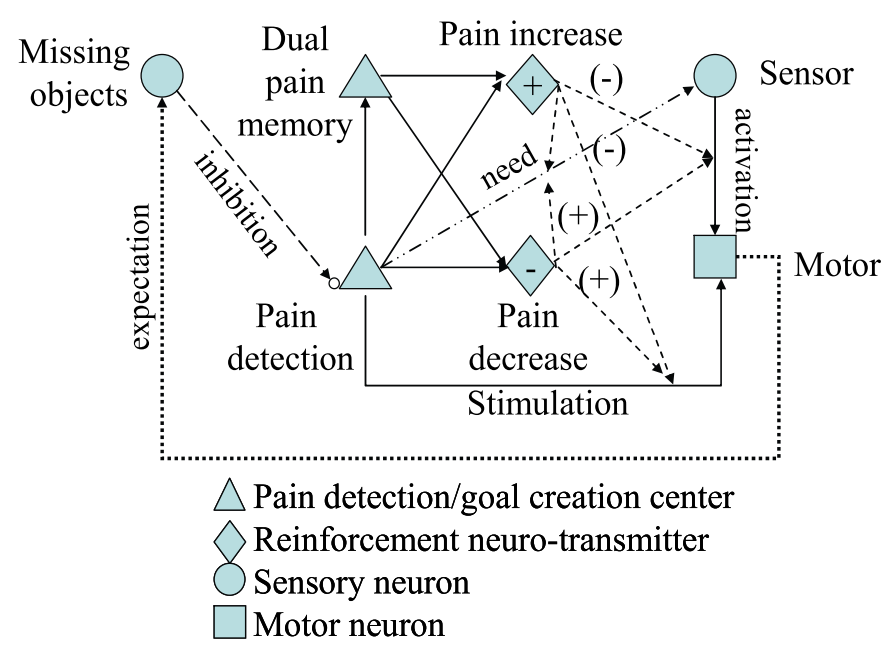
\includegraphics[width=0.7\linewidth]{rozdzial2/images/goal_creation_system_unit}
	\caption{Schemat podstawowego elementu systemu tworzenia celów. Źródło: 
	\cite{motivation_in_ei}.}
	\label{fig:goalcreationsystemunit}
\end{figure}

tu też tekst
